\chap{Flow and Error Control in Communication}
% https://www.youtube.com/watch?v=T-EVqAZ9SVU
% https://www.youtube.com/watch?v=JQbhxgPEhns
% https://youtu.be/teI6O4bFpD4
% https://youtu.be/FbjBUlM6p8g

\section{Introduction}
Flow control and Error control are the two main responsibilities of the data link layer, which is a communication channel for node-to-node delivery of the data. The functions of the flow and error control are explained as follows.\\

Flow control mainly coordinates with the amount of data that can be sent before receiving an acknowledgment from the receiver and it is one of the major duties of the data link layer. For most of the communications, flow control is a set of procedures that mainly tells the sender how much data the sender can send before it must wait for an acknowledgment from the receiver.\\

A critical issue, but not really frequently occurred, in the flow control is that the processing rate is slower than the transmission rate. Due to this reason each receiving device has a block of memory that is commonly known as buffer, that is used to store the incoming data until this data will be processed. In case the buffer begins to fill-up then the receiver must be able to tell the sender to halt the transmission until once again the receiver become able to receive.\\

Meanwhile, error control contains both error detection and error correction. It mainly allows the receiver to inform the sender about any damaged or lost frames during the transmission and then it coordinates with the re-transmission of those frames by the sender.\\

The term Error control in the communications mainly refers to the methods of error detection and re-transmission. Error control is mainly implemented in a simple way and that is whenever there is an error detected during the exchange, then specified frames are re-transmitted and this process is also referred to as Automatic Repeat request(ARQ).\\

The target in this lab is to implement a UART communication between the STM32 and a simulated terminal. A data request is sent from the terminal to the STM32. Afterward, computations are performed at the STM32 before a data packet is sent to the terminal. The terminal is supposed to reply an ACK to confirm the communication successfully or not.

\newpage
\section{Proteus simulation platform}

\begin{figure}[!htp]
    \centering
    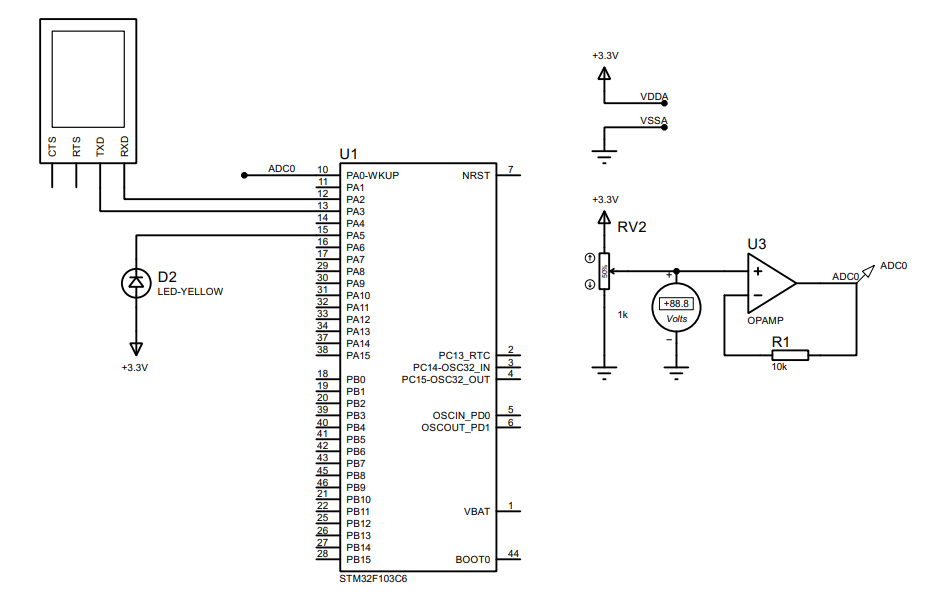
\includegraphics[width=5in]{source/picture/bai_6/Proteus_Simulation.PNG}
    \caption{\textit{Simulation circuit on Proteus}}
    \label{bai4_pic_button_schematic_0}
\end{figure}

Some new components are listed bellow:
\begin{itemize}
    \item Terminal: Right click, choose Place, Virtual Instrument, then select VIRTUAL TERMINAL.
    \item Variable resistor (RV2): Right click, choose Place, From Library, and search for the POT-HG device. The value of this device is set to the default 1k.
    \item Volt meter (for debug): Right click, choose Place, Virtual Instrument, the select DC VOLTMETER.
    \item OPAMP (U3): Right click, choose Place, From Library, and search for the OPAMP device.
\end{itemize}

The opamp is used to design a voltage follower circuit, which is one of the most popular applications for opamp. In this case, it is used to design an adc input signal, which is connected to pin PA0 of the MCU.\\

Double click on the virtual terminal and set its baudrate to 9600, 8 data bits, no parity and 1 stop bit, as follows:
\newpage
\begin{figure}[!htp]
    \centering
    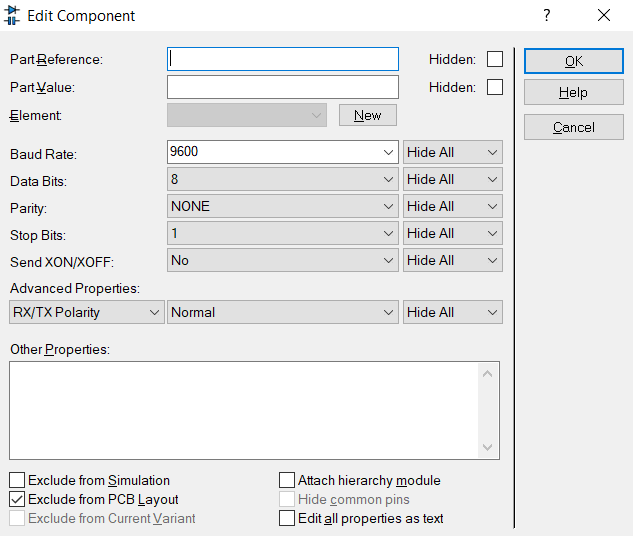
\includegraphics[width=4in]{source/picture/bai_6/Proteus_Simulation2.PNG}
    \caption{\textit{Terminal configuration}}
    \label{bai4_pic_button_schematic_0}
\end{figure}

\section{Project configurations}
A new project is created with following configurations, concerning the UART for communications and ADC input for sensor reading. The pin PA5 should be an GPIO output, for LED blinky.
\subsection{UART Configuration}
From the ioc file, select \textbf{Connectivity}, and then select the \textbf{USART2}. The parameter settings for UART channel 2 (USART2) module are depicted as follows:

\begin{figure}[!htp]
    \centering
    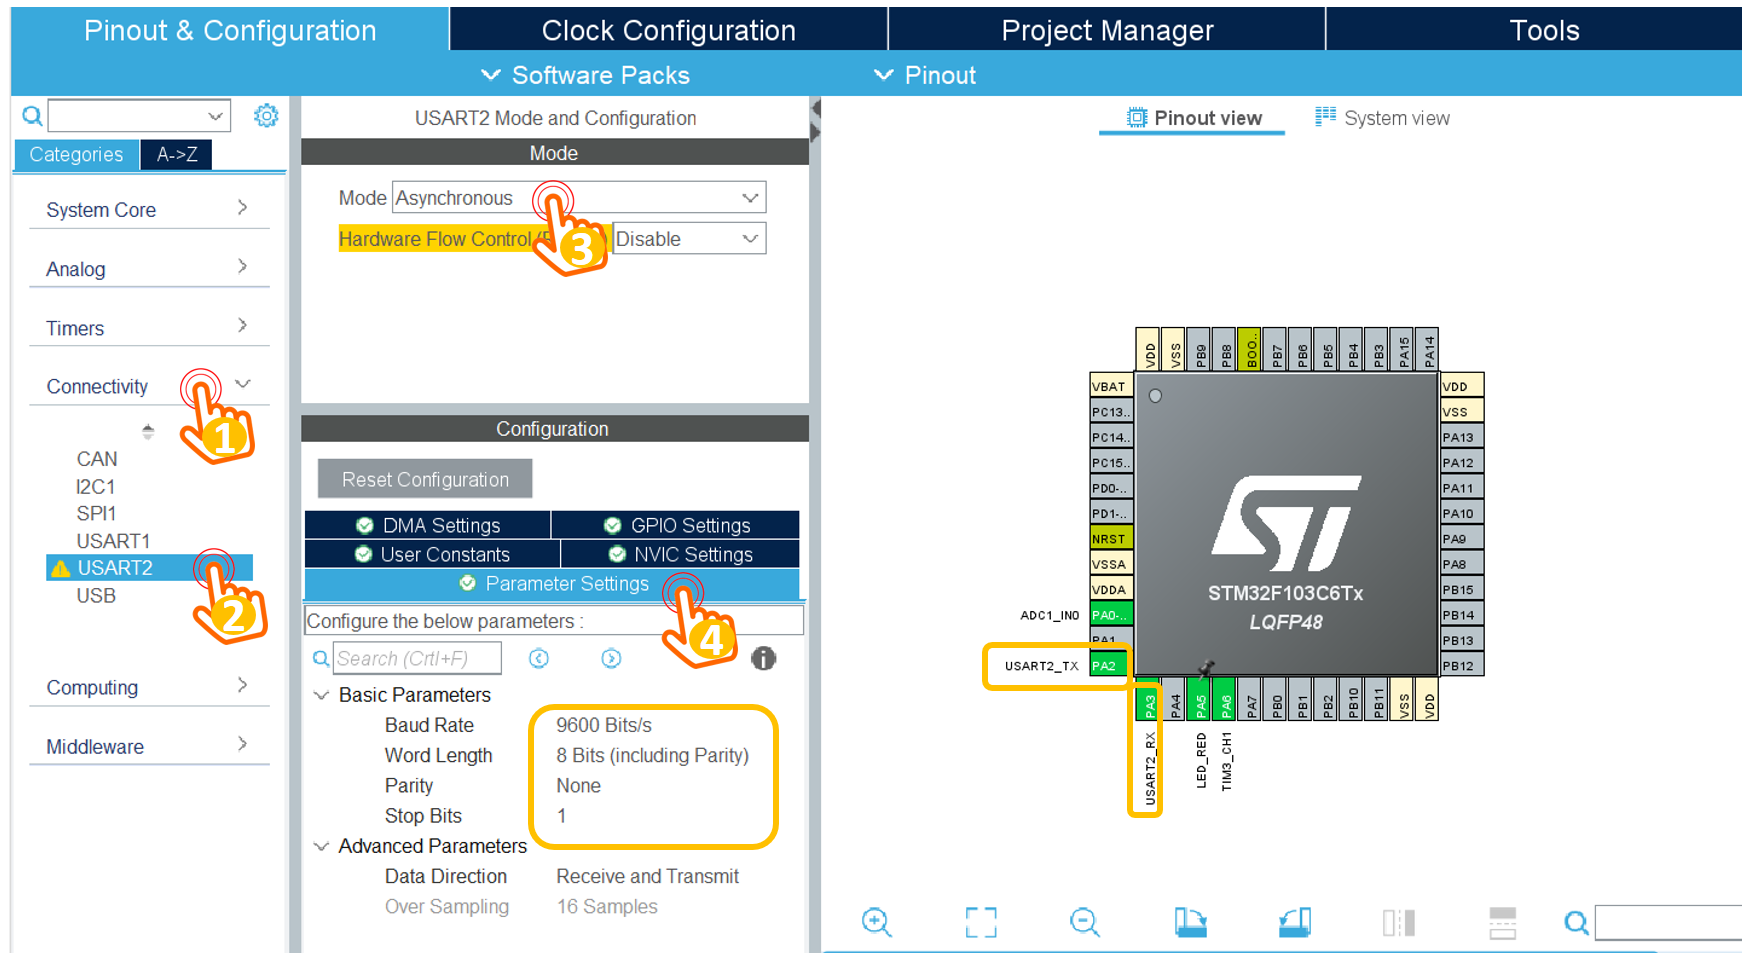
\includegraphics[width=4.5in]{source/picture/bai_6/stm32_uart_1.PNG}
    \caption{\textit{UART configuration in STMCube}}
    \label{1}
\end{figure}

The UART channel in this lab is the Asynchronous mode, 9600 bits/s with no Parity and 1 stop bit. After the uart is configured, the pins PA2 (Tx) and PA3(Rx) are enabled. \\

Finally, the NVIC settings are checked to enable the UART interrupt, as follows:
\begin{figure}[!htp]
    \centering
    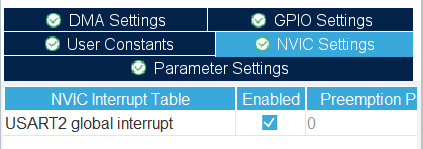
\includegraphics[width=3.5in]{source/picture/bai_6/stm32_uart_2.PNG}
    \caption{\textit{Enable UART interrupt}}
    \label{2}
\end{figure}

\subsection{ADC Input}
In order to read a voltage signal from a simulated sensor, this module is required. By selecting on \textbf{Analog}, then \textbf{ADC1}, following configurations are required:
\begin{figure}[!htp]
    \centering
    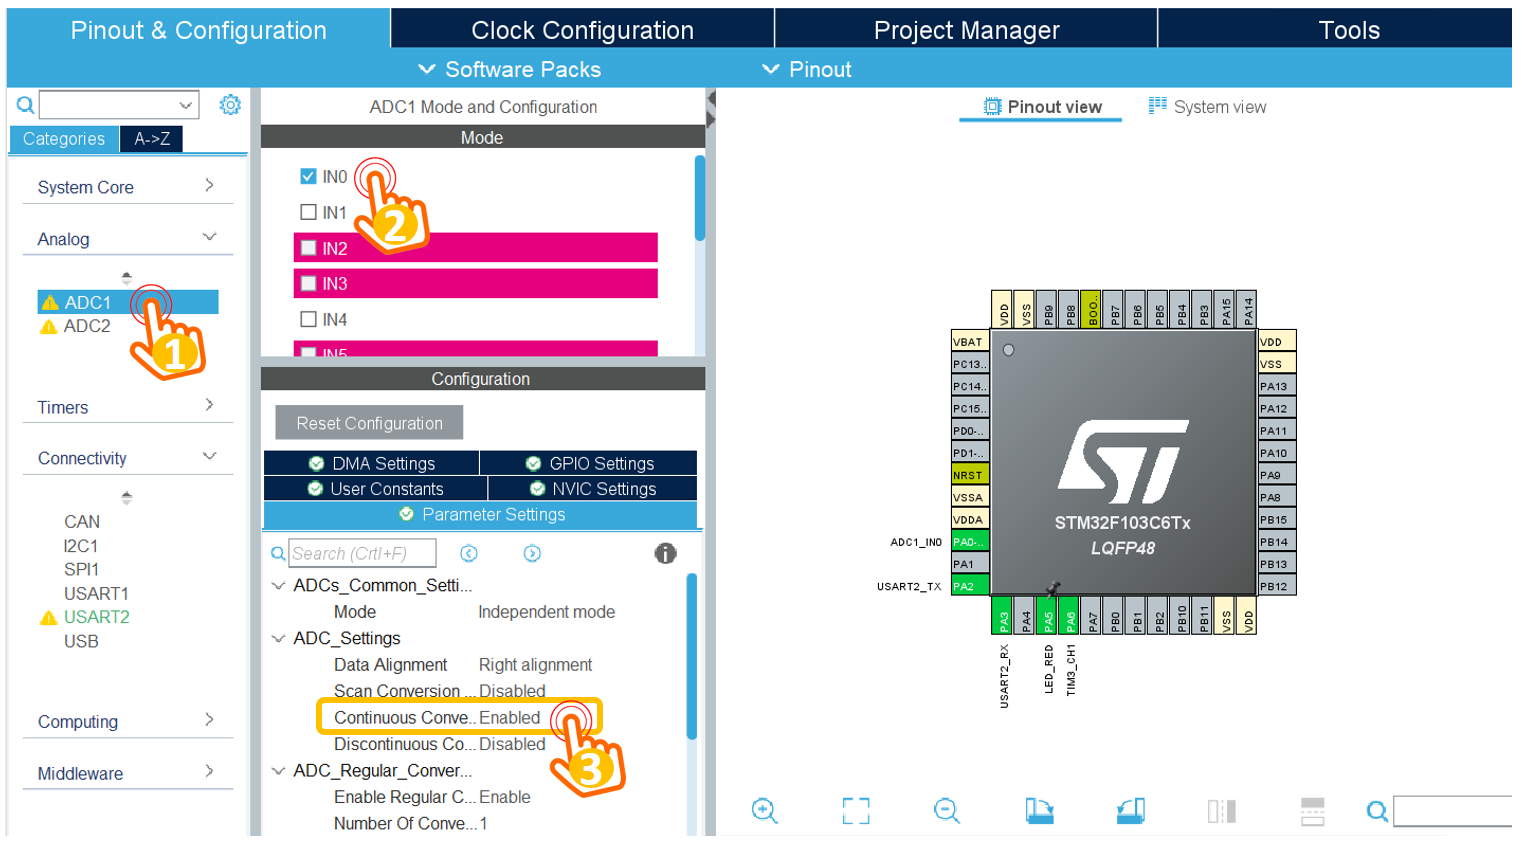
\includegraphics[width=4.5in]{source/picture/bai_6/stm32_adc_1.PNG}
    \caption{\textit{Enable UART interrupt}}
    \label{3}
\end{figure}

The ADC pin is configured to PA0 of the STM32, which is shown in the pinout view dialog. \\

Finally, the PA5 is configured as a GPIO output, connected to a blinky LED.

\section{UART loop-back communication}
This source is required to add in the main.c file, to verify the UART communication channel: sending back any character received from the terminal, which is well-known as the loop-back communication.

\begin{lstlisting}[caption= Implement the UART interrupt service routine]
/* USER CODE BEGIN 0 */
uint8_t temp = 0;

void HAL_UART_RxCpltCallback(UART_HandleTypeDef *huart){
	if(huart->Instance == USART2){
		HAL_UART_Transmit(&huart2, &temp, 1, 50);
		HAL_UART_Receive_IT(&huart2, &temp, 1);
	}
}
/* USER CODE END 0 */
\end{lstlisting}

When a character (or a byte) is received, this interrupt service routine is invoked. After the character is sent to the terminal, the interrupt is activated again. This source code should be placed in a user-defined section.\\

Finally, in the main function, the proposed source code is presented as follows:

\begin{lstlisting}[caption=Implement the main function]
int main(void)
{
  HAL_Init();
  SystemClock_Config();

  MX_GPIO_Init();
  MX_USART2_UART_Init();
  MX_ADC1_Init();

  HAL_UART_Receive_IT(&huart2, &temp, 1);

  while (1)
  {
	  HAL_GPIO_TogglePin(LED_RED_GPIO_Port, LED_RED_Pin);
	  HAL_Delay(500);
  }
  
}
\end{lstlisting}

\section{Sensor reading}
A simple source code to read adc value from PA0 is presented as follows:
\begin{lstlisting}[caption=ADC reading from AN0]
uint32_t ADC_value = 0;
while (1)
{
  HAL_GPIO_TogglePin(LED_RED_GPIO_Port, LED_RED_Pin);
  ADC_value =  HAL_ADC_GetValue(&hadc1);
HAL_UART_Transmit(&huart2, (void *)str, sprintf(str, "%d\n", ADC_value), 1000);
  HAL_Delay(500);
}
\end{lstlisting}

Every half of second, the ADC value is read and its value is sent to the console. It is worth noticing that the number ADC\_value is convert to ascii character by  using the sprintf function.\\

The default ADC in STM32 is 13 bits, meaning that 5V is converted to 4096 decimal value. If the input is 2.5V, ADC\_value is 2048.

\section{Project description}
In this lab, a simple communication protocol is implemented as follows:
\begin{itemize}
    \item From the console, user types \textbf{!RST\#} to ask for a sensory data.
    \item The STM32 response the ADC\_value, following a format \textbf{!ADC=1234\#}, where 1234 presents for the value of ADC\_value variable.
    \item The user ends the communication by sending \textbf{!OK\#}
\end{itemize}

The timeout for waiting the \textbf{!OK\#} at STM32 is 3 seconds. After this period, its packet is sent again. \textbf{The value is kept as the previous packet}.

\subsection{Command parser}
This module is used to received a command from the console. As the reception process is implement by an interrupt, the complexity is considered seriously. The proposed implementation is given as follows.\\

Firstly, the received character is added into a buffer, and a flag is set to indicate that there is a new data.

\begin{lstlisting}[caption= Add the received character into a buffer]
#define MAX_BUFFER_SIZE  30
uint8_t temp = 0;
uint8_t buffer[MAX_BUFFER_SIZE];
uint8_t index_buffer = 0;
uint8_t buffer_flag = 0;
void HAL_UART_RxCpltCallback(UART_HandleTypeDef *huart){
	if(huart->Instance == USART2){

		//HAL_UART_Transmit(&huart2, &temp, 1, 50);
		buffer[index_buffer++] = temp;
		if(index_buffer == 30) index_buffer = 0;

		buffer_flag = 1;
		HAL_UART_Receive_IT(&huart2, &temp, 1);
	}
}
\end{lstlisting}

A state machine to extract a command is implemented in the while(1) of the main function, as follows:
\begin{lstlisting}[caption= State machine to extract the command]
while (1){
    if(buffer_flag == 1){
        command_parser_fsm();
        buffer_flag = 0;
    }
}
\end{lstlisting}

The output of the command parser is to set \textbf{command\_flag} and \textbf{command\_data}. In this project, there are two commands, \textbf{RTS} and \textbf{OK}. The program skeleton is proposed as follows:
\begin{lstlisting}[caption= Program structure]
while (1){
    if(buffer_flag == 1){
        command_parser_fsm();
        buffer_flag = 0;
    }
    uart_communiation_fsm();
}
\end{lstlisting}

\subsection{Project implementation}
Students are proposed to implement 2 FSM in seperated modules. Students are asked to design the FSM before their implementations in STM32Cube.
